\chapter{対話型数値計算}

本章の目的は、
Pythonの対話型実行環境であるJupyter-notebookを用いてコンピュータによる数値計算を体感し、プログラミングの原理を実感することである。

Jupyter-notebookは、データ解析を簡単に実施できること、その結果を再利用かつ配布しやすい形で残すことができるため、現在急激に利用が広まっているソフトウェアである。

インストールも簡単であるため、各自のPCにもインストールすることを勧める。詳しくは、\ref{chap:anaconda}章を参照すること。

\section{Jupyter-notebookの起動}
Jupyte起動するためにコマンドプロンプトを実行する。
いくつか方法があるが「Winキー」+「R」を同時押しして「ファイル名から起動」を実行し、

\url{cmd}

\noindent を入力しEnterを押す方法が簡単である(図\ref{fig:Anaconda_launch1})。
コマンドプロンプトで

\url{jupyter-notebook}

\noindent を入力し実行すると(図\ref{fig:Anaconda_launch2})、
Jupyter-notebookのスタート画面が立ち上がる(図\ref{fig:Anaconda_launch3})。
 
\begin{figure}[htbp]
	\centering
	\fbox{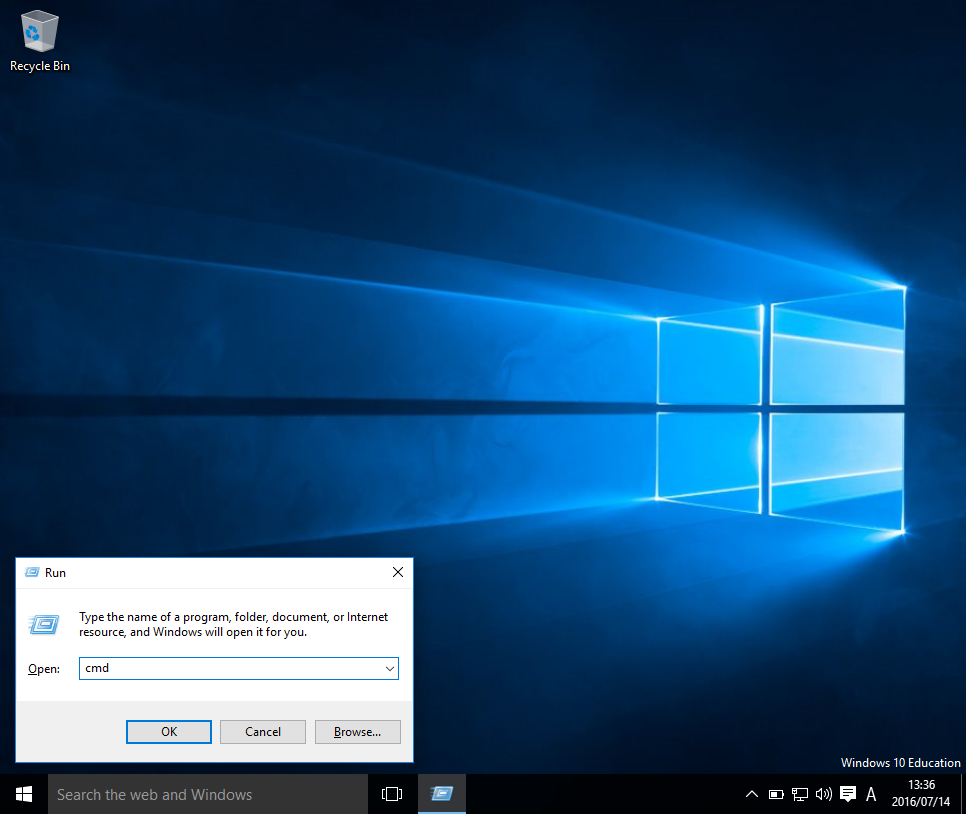
\includegraphics[width=10cm]{TeX_files/fig_python_install/Anaconda_launch1.png}}
	\caption{
		\label{fig:Anaconda_launch1}
		「Winキー」+「R」を押して出てくる検索窓に「cmd」を入力してEnterを押す。
			}
\end{figure}

\begin{figure}[htbp]
	\centering
	\fbox{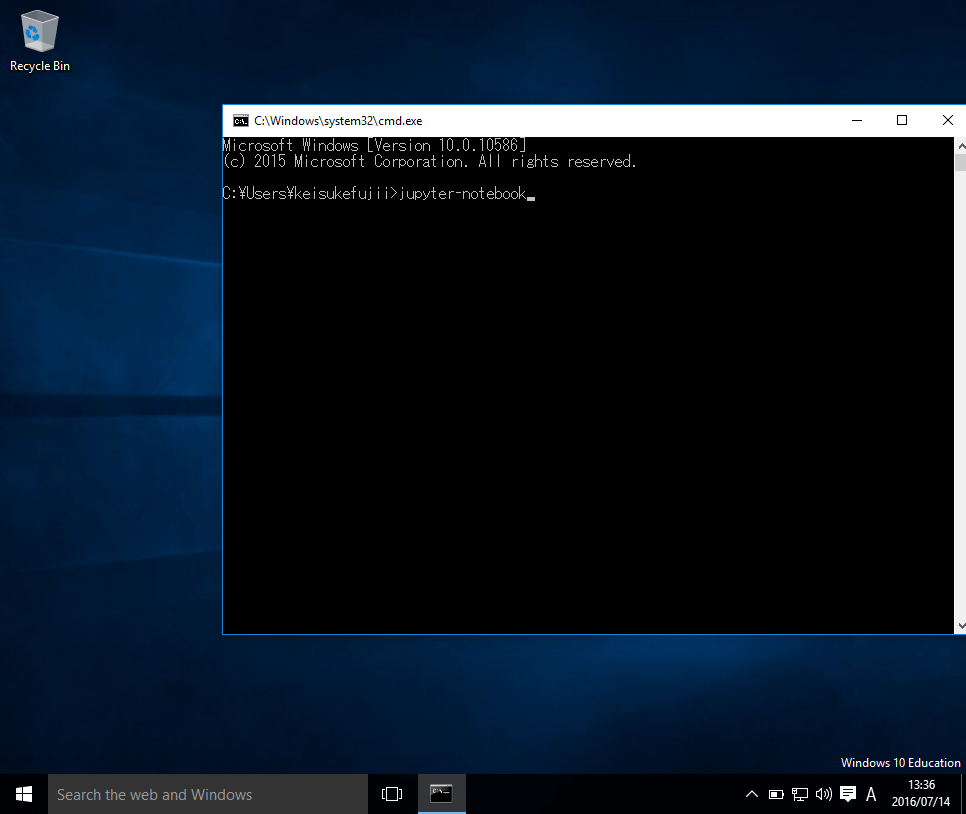
\includegraphics[width=10cm]{TeX_files/fig_python_install/Anaconda_launch2.png}}
	\caption{
		\label{fig:Anaconda_launch2}
		コマンドプロンプト内で「Jupyter-notebook」と入力し実行する。
	}
\end{figure}

\begin{figure}[htbp]
	\centering
	\fbox{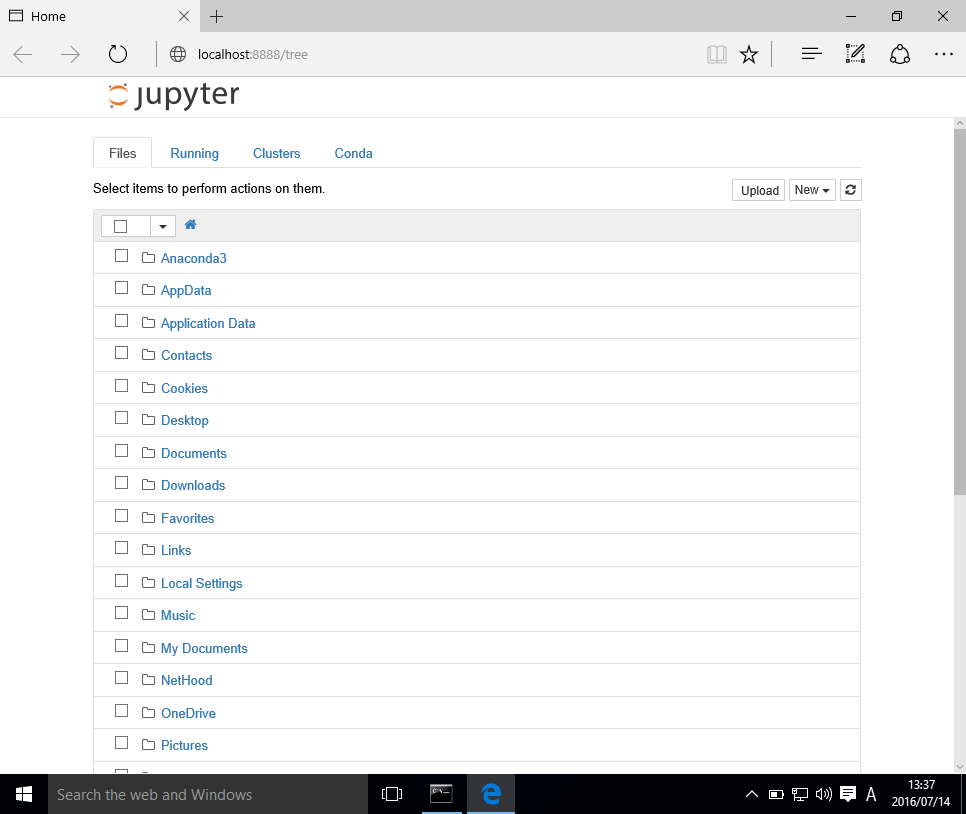
\includegraphics[width=10cm]{TeX_files/fig_python_install/Anaconda_launch3.png}}
	\caption{
		\label{fig:Anaconda_launch3}
		Jupyter-notebookの起動画面の一例。
	}
\end{figure}



% % % % % % % % % % % % % % % % % % % % % % % % % % % % % % % % % % % % % %


\section{Jupyer-notebookファイルの作成}
本演習を含め、将来的にはJupyter-notebookファイルを大量に作成することになる。
作成したファイルを見つけやすくするために、フォルダ構造を整理する。

マイドキュメント フォルダの中に、Johokiso-enshuフォルダを作成する。
マイドキュメントフォルダをクリックしその中に移動したあと、NewボタンからFolderをクリックする。
作成したフォルダの左側のチェックボックスをクリックすると出てくる renameボタンを押すことで名前の変更ができる(図\ref{fig:Jupyter_launch1})。

Johokiso-enshuフォルダ内に移動し、NewボタンからPython 3を起動する。
新しいウィンドウが開く(図\ref{fig:Jupyter_launch2})。



\begin{figure}[htbp]
	\centering
	\fbox{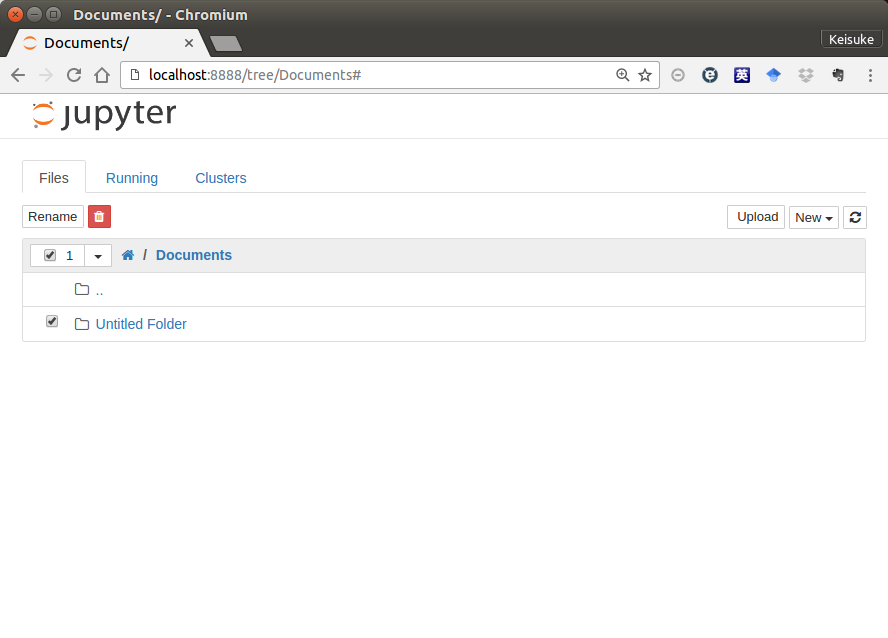
\includegraphics[width=10cm]{TeX_files/fig_python_install/Jupyter-launch1.png}}
	\caption{
		\label{fig:Jupyter_launch1}
		Jupyter-notebookでフォルダ構造を整理する。フォルダ名左横のチェックボックスを押すと、{\ttfamily rename}ボタンが出てくる。
	}
\end{figure}




% % % % % % % % % % % % % % % % % % % % % % % % % % % % % % % % % % % % % %

\section{Jupyter-notebookの基本的な使用方法}
\subsection{ノートブック名の変更}
新しいノートブックファイルには名前がまだつけられていないので、名前を変更する。
Jupyerロゴの横のUntitledをクリックすることで名を変更できる。
今日はプログラミング1回目なので Programming1-start とする(図\ref{fig:Jupyter1})。

\begin{figure}[htbp]
	\centering
	\fbox{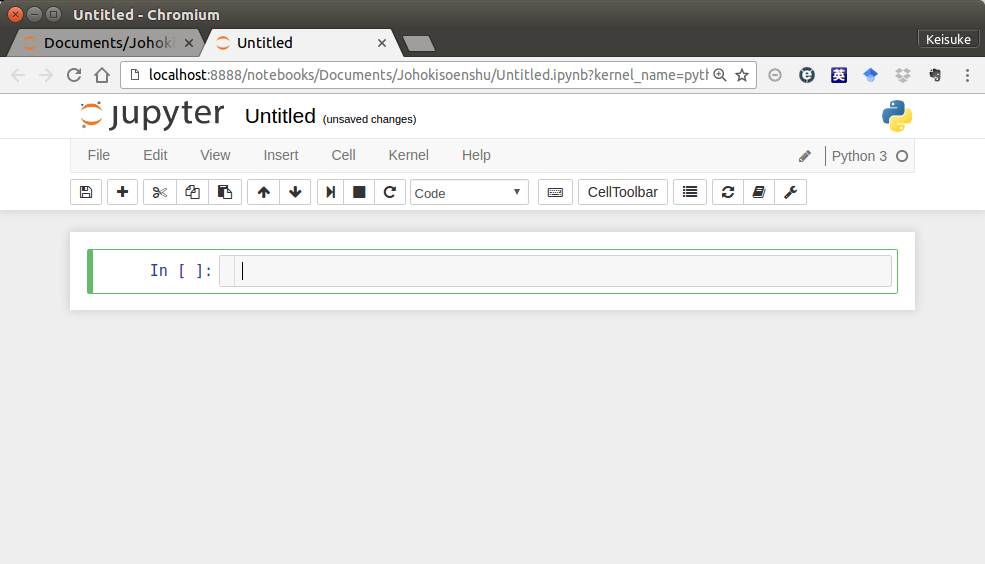
\includegraphics[width=10cm]{TeX_files/fig_python_install/Jupyter_launch2.png}}
	\caption{
		\label{fig:Jupyter_launch2}
		Jupyter-notebookで新しいPythonノートブックファイルを作成したときの様子。
	}
\end{figure}

\begin{figure}[htbp]
	\centering
	\fbox{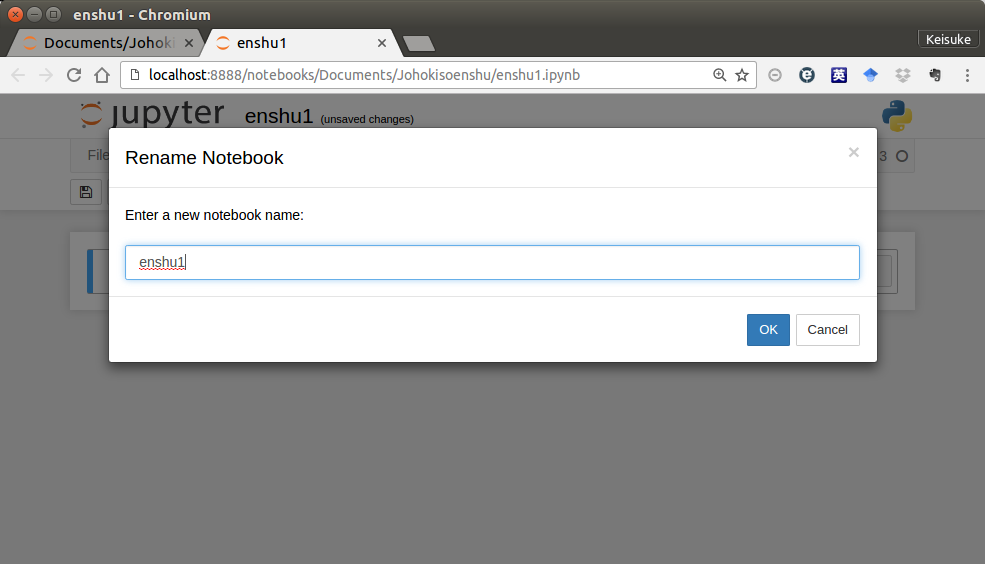
\includegraphics[width=10cm]{TeX_files/fig_python_install/Jupyter1.png}}
	\caption{
		\label{fig:Jupyter1}
		Jupyter-notebookファイルの名前を変更する。
	}
\end{figure}


% % % % % % % % % % % % % % % % % % % % % % % % % % % % % % % % % % % % % % % % % % % % % % % % % % % %

\subsection{Jupyter-notebookでの対話的プログラミング}
習うより慣れろということで、まずは命令(スクリプト)を実行させてみよう。
図\ref{fig:hello_world}にあるように、

{\ttfamily print('Hello world')}

\noindent
とセル内入力し、Shift + Enterの同時押しをするか、ツールバーの実行ボタンを押す。

エラーなく実行される場合、{\ttfamily Hello world'} とセルの下に表示されるはずである。
エラーがある場合は、図\ref{fig:hello_world_error}のように、セルの下にエラーメッセージが表示される。
このような場合は、再度正しいスクリプトを入力し、実行する。

\begin{figure}[htbp]
	\centering
	\fbox{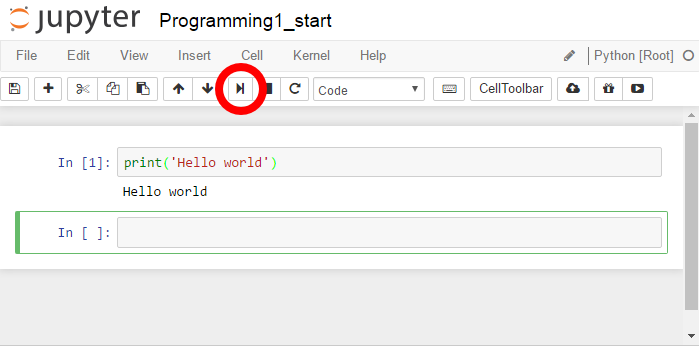
\includegraphics[width=8cm]{TeX_files/figs_jupyter_start/helloworld.png}}
	\caption{
		\label{fig:hello_world}
		{\ttfamily print('Hello world')} コマンドの実行画面
	}
\end{figure}
\begin{figure}[htbp]
	\centering
	\fbox{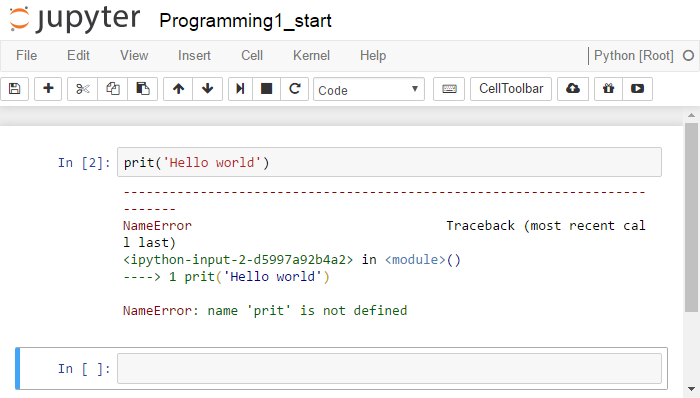
\includegraphics[width=8cm]{TeX_files/figs_jupyter_start/helloworld_error.png}}
	\caption{
		\label{fig:hello_world_error}
		コマンドを誤って入力した例。
	}
\end{figure}

この{\ttfamily print()}文は、カッコ内のものを画面に表示せよ、という命令である。
正しく入力できた時は、その結果が表示されていることがわかる。

% % % % % % % % % % % % % % % % % % % % % % % % % % % % % % % % % % % % % % % % % % % % % % % %

次に、図\ref{fig:python_start}のように一連の命令を実行してみよう。
\begin{figure}[htbp]
	\centering
	\fbox{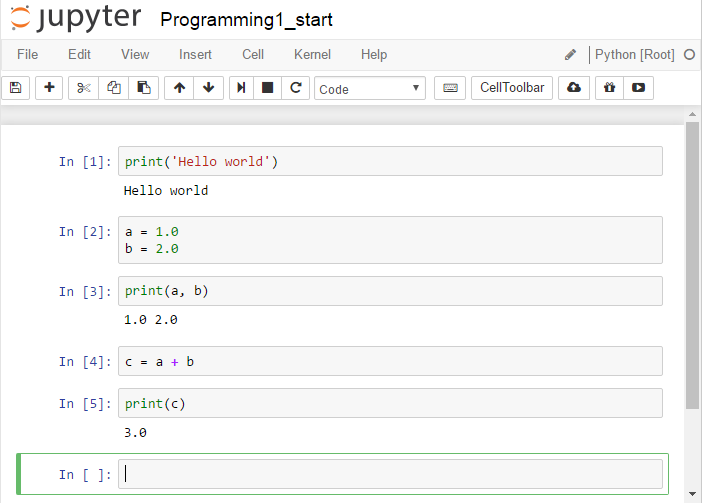
\includegraphics[width=8cm]{TeX_files/figs_jupyter_start/python_start.png}}
	\caption{
		\label{fig:python_start}
		{\ttfamily Hello world} 一連の命令を実行させた例。
	}
\end{figure}

\begin{itemize}
\item {\ttfamily a = 1.0, b = 2.0} 	

変数{\ttfamily a} に値1.0 を、変数{\ttfamily b}に値2.0 を代入する。

\item {\ttfamily print(a, b)} 	

変数{\ttfamily a, b} の値を表示する。

\item {\ttfamily c = a + b} 	

変数{\ttfamily c}に{\ttfamily a + b}を計算した結果を代入する。

\item {\ttfamily print(c)} 	

変数{\ttfamily c}の値を表示する。


\end{itemize}
\noindent
命令の内容は後で学ぶ。今は、コンピュータに命令をし、その命令が正しければコンピュータがそれを実行することがわかれば十分である。

\begin{comment}

\end{comment}
% % % % % % % % % % % % % % % % % % % % % % % % % % % % % % % % % % % % % % % % % % % % % % % % % % % %

\subsection{セルタイプ〜Code,Markdown〜}
Jupyter-notebookのセルには、{\ttfamily Code, Markdown、Raw NBConvert}の3状態がある。
これは、画面上部メニューの{\ttfamily Cell -> Cell Type}から設定できる(図\ref{fig:Cell_type})。
\begin{itemize}
\item {\ttfamily Code}状態は、上記のようなコンピュータへの命令を記入するためのもの、
\item {\ttfamily Markdown}状態は、命令以外の文章、特にコードの説明を記入するものである。
\end{itemize}

\noindent
{\ttfamily Code}状態はコンピュータへの命令内容を記述するためにもちろん重要であるが、
{\ttfamily Markdown}状態も、後でノートブックの内容を理解するために重要である。

Markdownセルを作成し、図\ref{fig:markdown}と同じ内容を記入して実行してみよ。


\begin{figure}[htbp]
	\centering
	\fbox{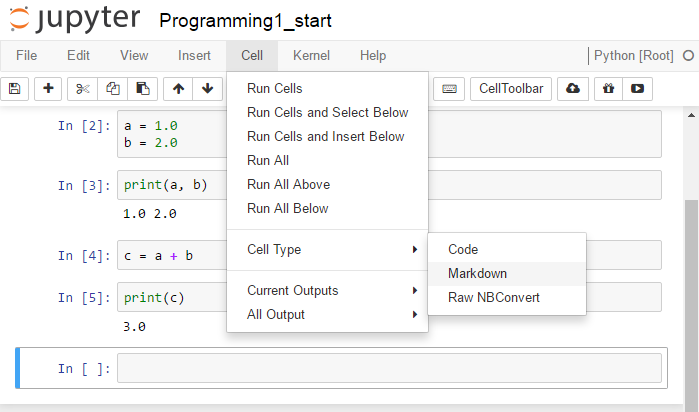
\includegraphics[width=8cm]{TeX_files/figs_jupyter_start/cell_type.png}}
	\caption{
		\label{fig:Cell_type}
		セルタイプを変更する様子。
	}
\end{figure}
\begin{figure}[htbp]
	\centering
	\fbox{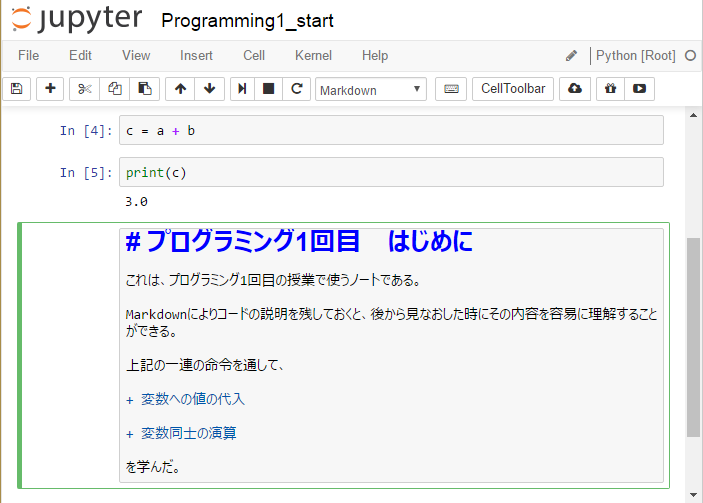
\includegraphics[width=8cm]{TeX_files/figs_jupyter_start/markdown.png}}
	\caption{
		\label{fig:markdown}
		Markdownセルに入力している様子。
	}
\end{figure}




% % % % % % % % % % % % % % % % % % % % % % % % % % % % % % % % % % % % % % % % % % % % % % % % % % % %

\subsection{Jupyter-notebookファイルの保存}
Jupyter-notebookファイルを保存するためには、左上の{\ttfamily File -> Save and Checkpoint}を選ぶか、
単純に左側のフロッピーディスクボタンをクリックする。

\subsection{Jupyter-notebookの終了}
上で作成したJupyter-notebookを保存し、ブラウザを閉じよ。
しかし実は、ブラウザを閉じただけでは実はソフトウェアは終了していない。
特に、ファイル一覧の画面で色がついたノートブックファイルは現在実行中のものを示している。

Jupyter-notebookを完全に終了させるためには、コマンドプロンプドに戻り、Ctrl+Cを押す。

% % % % % % % % % % % % % % % % % % % % % % % % % % % % % % % % % % % % % % % % % % % % % % % % % % % %
\begin{comment}
\subsection{編集モード・コマンドモード}
Jupyter-notebookには{\ttfamily 編集モード、コマンドモード}の2つのモードがある。

セル内をクリックすると文字入力が可能となる。
この時、セルの左側は緑色になるが、
これが編集モードであり、各種命令文を打ち込むことが可能である。

セル外をクリックすると、セルの左側が青色のコマンドモードになる。
この時は命令を打ち込むことはできず、その代わりキーボードからの入力が

\begin{itemize}
\item コマンドモード
セルのサイドが青くなる。文字入力はできない。
セル内をクリックするか、Enterキーを押すことで編集モードに移行できる。
このモードではショートカットでいろいろな操作が可能である。
このモードで {\ttfamily h} キーを押すことでその一覧を見ることができる。
\item 編集モード

\end{itemize}

% % % % % % % % % % % % % % % % % % % % % % % % % % % % % % % % % % % % % % % % % % % % % % % % % % % %
\section{Jupyter-notebookの活用例\label{sec:jupyter_example}}

内容の詳しい説明は後に述べることとして、実際の活用例に近いものを作成してみよう。

Jupyter-notebookを再度起動し、新しくノートブックファイルを作成する。
ファイル名は{\ttfamily Programming1-example}としておこう。
そのノートブック内で、図\ref{fig:jupyter_application}に示す一連の命令を実行せよ。

これは、物理学実験などで得られた(仮想的な)データの内容の記録、およびその可視化を行っている例である。
Jupyter-notebookでは、データがどのようにして得られたか、どのように解析したかやその結果を記録することができる。
このような情報を残しておくことで、レポート作成をスムースに行うことができる。

\begin{figure}[htbp]
	\centering
	%\fbox{\includegraphics[width=8cm]{TeX_files/figs_jupyter_start/jupyter_application.png}}
	\caption{
		\label{fig:jupyter_application}
		{\ttfamily Hello world} 一連の命令を実行させた例。
	}
\end{figure}



% % % % % % % % % % % % % % % % % % % % % % % % % % % % % % % % % % % % % % % % % % % % % % % % % % % %

\end{comment}